\documentclass[letterpaper,conference]{IEEEtran}

\usepackage{cite}
\usepackage{amsmath,amssymb}
\usepackage{booktabs}
\usepackage{graphicx}
\usepackage{placeins}
\usepackage{balance}
\usepackage{array}
\usepackage{url}

\graphicspath{{figures/}}
\DeclareGraphicsExtensions{.pdf,.png}

\title{AERIS: Reliable Routing for Wireless Sensor Networks under Heterogeneous Channels}

\author{
\IEEEauthorblockN{Kangrui Li, Junyi Lin, and Xiaobo Zhang}
\IEEEauthorblockA{
Faculty of Automation, Guangdong University of Technology \\
Guangzhou 510006, China \\
\textit{Corresponding author:} Kangrui Li \\
\texttt{1403073295@mails.gdut.edu.cn}
}
}

\begin{document}

\maketitle

\begin{abstract}
AERIS is a rule-based hierarchical routing protocol for wireless sensor networks under heterogeneous channels. We compare it with LEACH, PEGASIS, HEED, and TEEN in a corrected canonical NS-3 study across four environments and 100, 500, and 1000 nodes ($n=30$ per environment-node-protocol cell) and in a strict-physics simulator with explicit collision and relay stress ($n=3200$ per cell). The environment ordering is stable across both layers: PEGASIS leads in indoor office, whereas AERIS leads in indoor factory, outdoor suburban, and outdoor urban. In corrected NS-3 at 1000 nodes, AERIS reaches 0.593, 0.770, and 0.200 in those three harsher environments, compared with 0.324, 0.549, and 0.019 for PEGASIS. A corrected 400-replicate mechanism study shows that the gain is carried mainly by Gateway-assisted uplinks, while first-node death falls to 1--4.5 rounds in most harsh 500/1000-node cells. For the settings studied here, AERIS is preferable when delivery dominates, whereas PEGASIS remains preferable in benign or lifetime-dominated regimes.
\end{abstract}

\begin{IEEEkeywords}
wireless sensor networks, reliable routing, cross-platform evaluation, deployment boundary
\end{IEEEkeywords}

\section{Introduction}
Wireless sensor network (WSN) routing is usually discussed in terms of energy, yet in many deployments link stability matters just as much \cite{tossa2025wireless,thakur2025ai-driven,almutairi2024survey}. This becomes clear when classical protocols are placed side by side: LEACH emphasizes clustered forwarding \cite{heinzelman2000leach}, PEGASIS uses chain-based aggregation \cite{lindsey2002pegasis}, HEED relies on residual-energy-aware head election \cite{younis2004heed}, and TEEN reports only when event thresholds are crossed \cite{manjeshwar2001teen}. Real links make the trade-off harder because low-power WSN channels are environment sensitive and often unstable near connectivity thresholds; recent LCN and sensor-network work continues to study link-quality prediction, corrupted-packet recovery, and interference resilience for this reason \cite{chatharajupalli2025probing,szafranski2025cec,xu2025sloraplus}.

This leads to a practical question: when do simple, auditable control rules outperform classical energy-first designs under harsh channels, and what is the price of that reliability gain? AERIS addresses this question with fixed-rule control rather than learned routing. Its design combines Context-Adaptive Switching (CAS) for intra-cluster mode selection, Gateway reinforcement for CH-to-BS uplinks, and a sparse Skeleton fallback backbone.

We make three contributions. First, we present AERIS as a fixed-rule routing design whose online behavior can be traced directly to channel and topology inputs. Second, we evaluate AERIS with a corrected canonical five-protocol NS-3 comparison and a stricter simulator matrix, keeping baseline ranking separate from stress evidence. Third, we use ablation, pooled trade-off statistics, and a corrected mechanism study to show that the observed gain comes mainly from Gateway support and is paid for through earlier node death.

\section{Related Work}
Classical low-overhead WSN protocols still define the main engineering operating points. LEACH and HEED reduce long-range transmission burden through clustering, but their uplink quality is still sensitive to head placement and channel degradation \cite{heinzelman2000leach,younis2004heed}. PEGASIS spreads load through chain forwarding but pays for that robustness with long routes and serialization \cite{lindsey2002pegasis}. TEEN reduces redundant transmissions under threshold-triggered sensing, but its reporting logic makes metric interpretation sensitive to how ``expected'' delivery is defined \cite{manjeshwar2001teen}. These protocols span the basic reliability-energy-latency trade-offs that any new design has to face.

Recent work has improved reliability through learning, hybrid control, or deployment adaptation \cite{ren2024mefi,okine2024multi-agent,hu2024security,pushpa2025optimizing,jain2025optimized,elfouly2023environment-aware,dan2024accuracy-aware,bhukya2025hybrid,tossa2025wireless,singh2025enhanced,wang2024energy-efficient,zhang2025energy,manogaran2025developing,juwaied2025dl-heed}. AERIS is closer to this line of work than to purely energy-minimizing clustering, but it keeps the runtime logic deliberately simple: fixed coefficients, explicit control paths, and no training-time dependence. Recent 2024--2026 studies have also sharpened the surrounding context by surveying LLN path-finding requirements \cite{almutairi2024survey}, SDN-style management over IoT/LLN deployments \cite{djennadi2025exploring}, AI-driven energy-efficient routing in IoT-enabled WSNs \cite{thakur2025ai-driven}, and RPL-family objective functions for industrial IoT and LLN routing \cite{brito2026ec,habib2026edcc,cheppali2025hybrid}. Recent LCN papers point to adjacent deployment pressures in position- and energy-aware LoRa routing, energy-aware scheduling, RSSI-based link prediction, and corrupted LoRa packet recovery \cite{udugampola2025position,dorval2025energy,chatharajupalli2025probing,szafranski2025cec}. Broader families such as CTP, RPL/ORPL/ORW, coding-based reliability, and channel-hopping systems are also relevant. They are outside the current evidence package because this paper is centered on a corrected comparison against classical WSN baselines, not because they are unimportant in practice.

That scope is intentional. Classical protocols are still the clearest reference point for showing how a new design moves the balance between delivery, energy, and lifetime, but the paper should not be read as a comparison against the full space of low-power routing systems. Collection and RPL-style protocols matter for deployment realism; recent LLN surveys and RPL studies also emphasize the unresolved issues around scalable path selection, topology management, and heterogeneous control in these networks \cite{almutairi2024survey,djennadi2025exploring,brito2026ec,habib2026edcc,cheppali2025hybrid}; coding-based reliability and channel-hopping matter when the stack can afford heavier coordination; opportunistic schemes matter when local diversity is high enough to justify more complex forwarding logic. AERIS is narrower than those routes. Its value proposition is that a simpler control path can still buy measurable reliability in the regimes studied here.

\begin{figure*}[t]
\centering
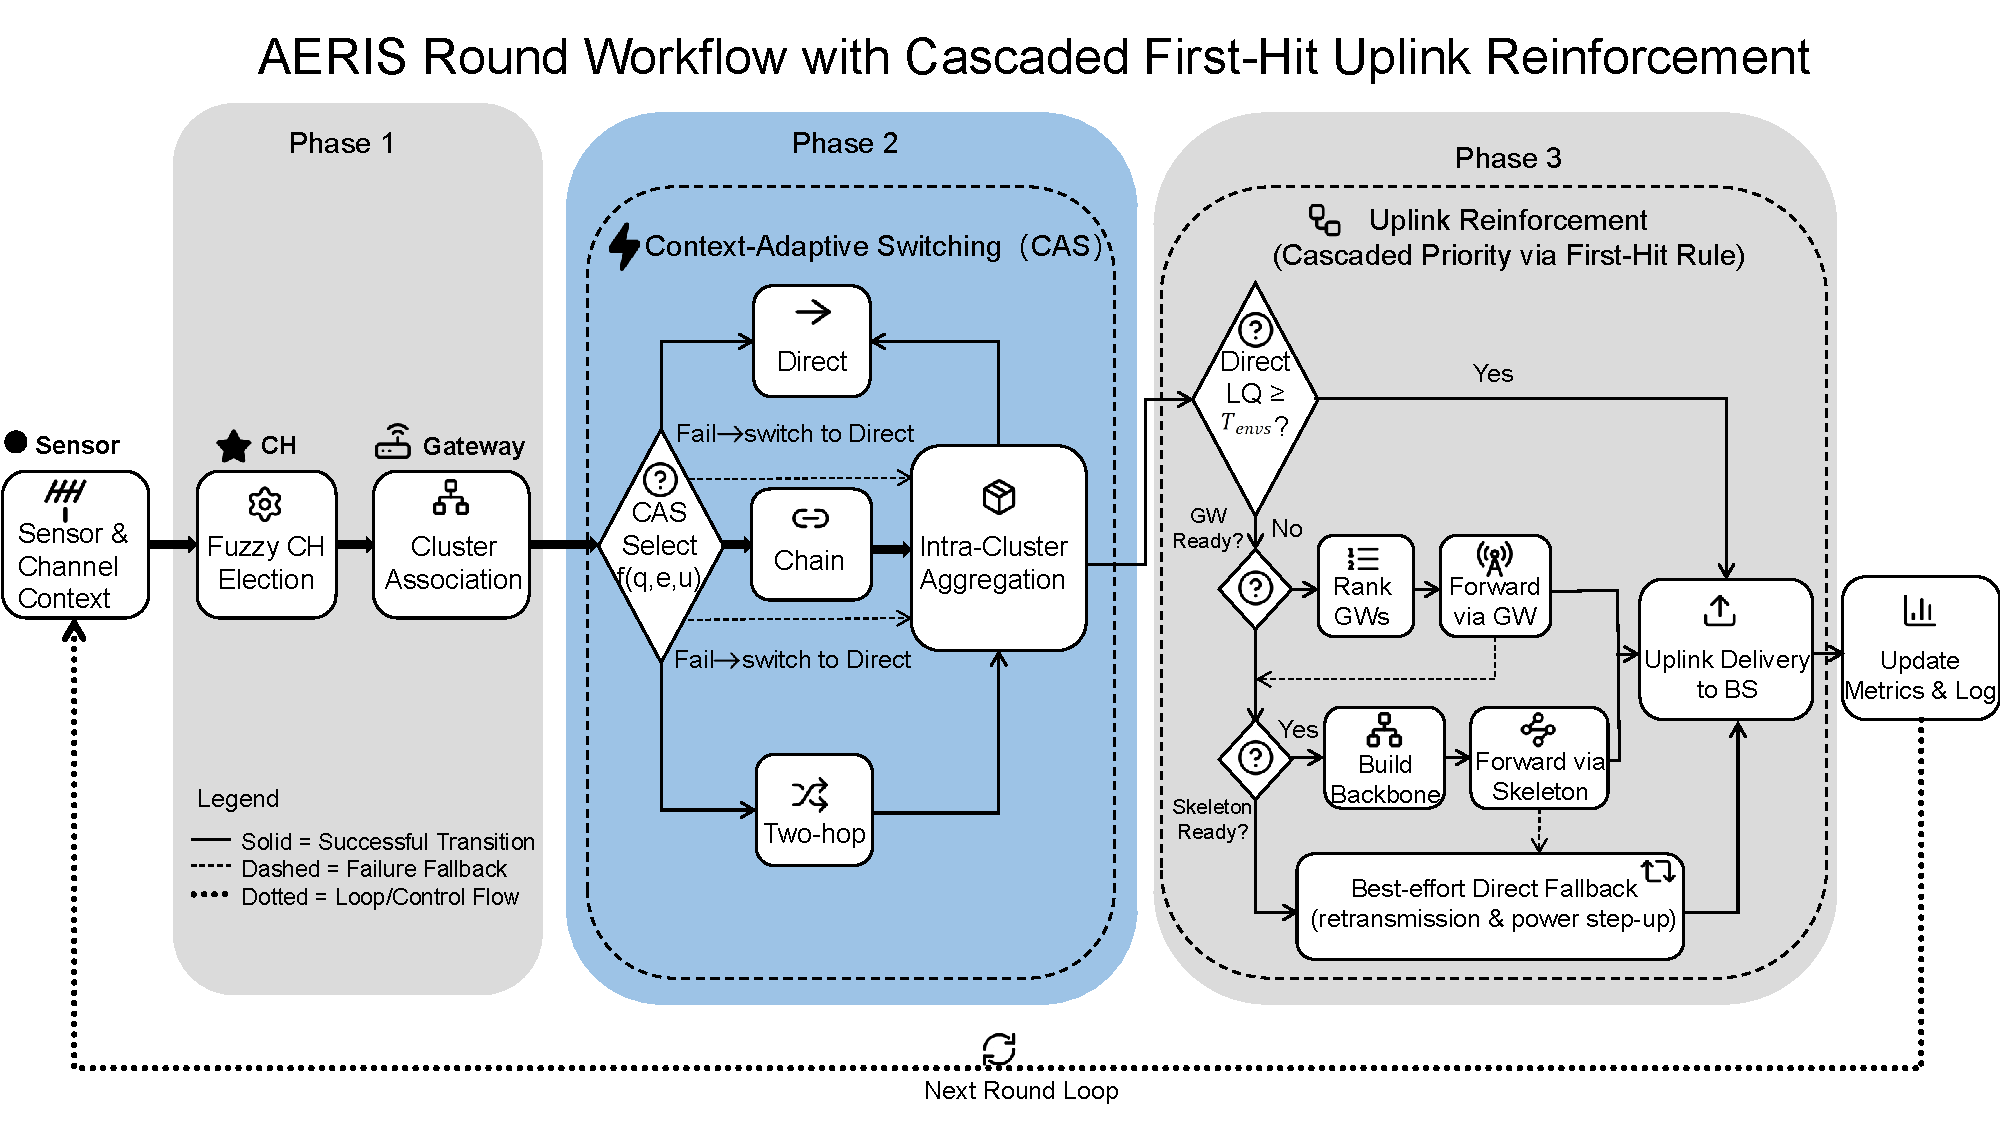
\includegraphics[width=0.90\textwidth]{fig0_aeris_workflow_temp_20260420.pdf}
\caption{AERIS round workflow with cascaded uplink reinforcement.}
\label{fig:aeris_workflow}
\end{figure*}

\section{Protocol Design}
AERIS combines CAS for intra-cluster transmission mode selection, Gateway reinforcement for cluster-head to base-station uplinks, and Skeleton forwarding for sparse CH fallback routes. The goal is to add reliability support only where direct forwarding becomes unreliable, while keeping online logic deterministic and auditable.

Gateway candidates are ranked by a fixed linear score,
\begin{equation}
\mathrm{Score}_i = \alpha \hat{E}_i + \beta \hat{C}_i + \gamma \hat{L}_i + \delta \hat{D}_i,
\end{equation}
where $\hat{E}_i$, $\hat{C}_i$, $\hat{L}_i$, and $\hat{D}_i$ denote normalized residual energy, centrality, link quality, and CH-to-BS distance. In this implementation, centrality is a distance-aware neighborhood surrogate computed from local geometry, link quality is the current channel-estimated success probability for the candidate hop, and all scalar features are normalized to $[0,1]$ before scoring. CAS uses another fixed linear rule over \{direct, chain, two-hop\}; the shared coefficients are held constant across environments in publication-tier runs, so mode selection is reproducible under identical inputs and seeds:
\begin{equation}
m^{\star}=\arg\max_{m \in \{\mathrm{direct},\mathrm{chain},\mathrm{two\mbox{-}hop}\}} \left( a_m \hat{q} + b_m \hat{e} + c_m \hat{u} \right),
\end{equation}
where $\hat{q}$, $\hat{e}$, and $\hat{u}$ are normalized local channel quality, residual energy, and utilization terms, and the coefficients $\{a_m,b_m,c_m\}$ are fixed for each candidate mode. Skeleton forwarding is built as a sparse CH relay backbone after clustering and is refreshed round-by-round together with the CH set, but the corrected publication configuration later shows that it acts as a reserve fallback path rather than an actively exercised mechanism in the audited runs.

The forwarding logic is cascaded rather than multipath. A cluster head first checks direct uplink quality, then tries Gateway support if available, then Skeleton support if available, and finally makes one last direct attempt. In the strict-physics regime, this ``best-effort direct fallback'' is a single direct transmission attempt without protocol-level retransmission.

In practice, the protocol only activates extra forwarding structure after a direct path has become unattractive under the current channel estimate. CAS decides whether a sensor-to-CH transfer stays direct, switches to a short chain, or uses a two-hop relay; Gateway support then targets the more fragile CH-to-BS segment; Skeleton remains a reserve fallback if Gateway support is unavailable. The control path is deliberately narrow: AERIS does not search a large policy space online, and the same inputs always trigger the same routing decisions.

AERIS is an engineering design rather than a formal routing theorem. It adds alternate forwarding structure only when the direct path looks weak, reacts to a small number of local conditions with fixed rules, and is therefore judged by how that choice changes delivery and cost in deployment.

\subsection{Why the Modules Are Ordered This Way}
The ordering of the modules is part of the design rather than an implementation detail. Direct transmission is checked first because it is the cheapest option whenever the channel still supports it. Gateway support comes next because the audited experiments show that the CH-to-BS segment is usually the first place where reliability collapses in harsher cells. Skeleton forwarding is deliberately placed behind Gateway support because it is intended to preserve a fallback path, not to replace the main uplink rule.

This ordering also keeps the policy interpretable. AERIS does not ask every round whether all possible forwarding structures should be explored. Instead, it asks a smaller sequence of questions: is direct transmission still reasonable, is there a nearby Gateway that can protect the uplink, and if not, does the sparse Skeleton path exist? The protocol therefore behaves like a controlled escalation path rather than a broad route search.

\subsection{Intended Operating Regime}
The design is aimed at deployments where channel quality varies significantly across the field and where a modest increase in runtime complexity is acceptable if it stabilizes delivery. It is not aimed at the cleanest office-like regimes, where the longest-lived chain often remains the better choice, and it is not aimed at routing stacks that can afford heavier control traffic or training-time optimization. This intended operating regime is important in reading the evaluation, because it explains why the paper compares AERIS against classical baselines but interprets the result as deployment guidance rather than universal ranking.

\section{Evaluation Setup}
The primary metric is packet delivery ratio over expected application-layer transmissions,
\begin{equation}
\mathrm{PDR}_{\mathrm{expected}}=\frac{N_{\mathrm{delivered}}}{N_{\mathrm{expected}}},
\end{equation}
where $N_{\mathrm{expected}}$ counts one packet per alive source node per round even if a protocol suppresses actual transmission. This denominator is kept fixed across protocols so that the reliability comparison is not quietly changed by protocol-specific reporting logic.

We use two complementary settings. The first is a corrected canonical NS-3 comparison against native AERIS, LEACH, PEGASIS, HEED, and TEEN implementations across four environments and 100, 500, and 1000 nodes ($n=30$ per environment-node-protocol cell). The second is a strict-physics Python simulator matrix across four environments and 100--1000 nodes ($n=3200$ per environment-node-protocol cell) with explicit collision and relay stress; in that layer, LEACH, HEED, and TEEN are reported in minimally adapted relay-enabled form for multi-hop comparability. The NS-3 study anchors the main ranking claim, whereas the strict matrix tests whether that conclusion survives under stronger deployment assumptions. To avoid relying on PDR alone, we also report total energy, lifetime, first-node death, and hop count in the frozen 100-node publication block. Module and trade-off analysis use that block together with a corrected 400-replicate AERIS mechanism matrix.

The four environments are used consistently across all experiments: indoor office, indoor factory, outdoor suburban, and outdoor urban. They are meant to cover a progression from relatively benign links to much harsher settings. The node counts then separate small-network behavior from the denser cells where poor CH-to-BS links and relay pressure become more visible.

This role split is deliberate. The canonical NS-3 study asks how AERIS compares to native classical baselines on an independent platform. The strict-physics simulator then tests whether that ordering survives under stronger relay and collision assumptions in an adapted stress layer rather than in a second canonical ranking layer, while lifetime, first-node death, hop count, and total energy show whether delivery gains come from spreading or concentrating load. Keeping these layers separate is one of the main repairs made after the earlier review cycle.

\begin{table}[t]
\caption{Experimental settings used in the paper.}
\label{tbl:exp_settings}
\centering
\scriptsize
\setlength{\tabcolsep}{3pt}
\begin{tabular}{lcccc}
\toprule
Layer & Platform & Protocols & Cells & Role \\
\midrule
Canonical & NS-3 & native 5-protocol & $4 \times 3$ & ranking \\
Strict & Python & adapted 5-protocol stress & $4 \times 6$ & stress \\
Mechanism & Python & AERIS-only grid & $4 \times 3$ & attribution \\
Frozen block & pooled stats & 5-protocol summary & 100-node only & trade-off \\
\bottomrule
\end{tabular}
\end{table}
\section{Results}
\subsection{Canonical NS-3 Results}
Figure~\ref{fig:ns3_canonical} gives the main ranking result because it uses canonical NS-3 baselines. PEGASIS is best in indoor office, while AERIS leads in factory, suburban, and urban conditions. In office, the corrected rerun is no longer an implausibly flat line: PEGASIS drops from 0.999953 at 100 nodes to 0.998690 at 1000 nodes, while AERIS stays near 0.920, 0.913, and 0.912 at the same scales.

The other three environments behave differently. At 1000 nodes in corrected NS-3, AERIS reaches 0.593 in indoor factory, 0.770 in outdoor suburban, and 0.200 in outdoor urban. The corresponding PEGASIS means are 0.324, 0.549, and 0.019, while LEACH, HEED, and TEEN remain lower still. The same ordering appears at 100 and 500 nodes as well.

What matters is that the boundary appears early. AERIS already leads in the harsher environments at 100 nodes and keeps that lead as the network becomes denser, while office remains the visible counterexample.

\begin{figure}[t]
\centering

\includegraphics[width=\columnwidth]{fig_lcn26_ns3_canonical_compact.pdf}
\caption{Corrected canonical five-protocol NS-3 comparison across four environments and 100, 500, and 1000 nodes ($n=30$ per cell). This is the main ranking figure because it uses native baselines on the independent NS-3 platform.}
\label{fig:ns3_canonical}
\end{figure}

Canonical NS-3 therefore supports a narrower but cleaner claim: AERIS is stronger in harsher channels, whereas PEGASIS is decisively better in benign office-like conditions. The result no longer depends only on the custom Python simulator, and the office cell acts as a built-in negative control against overclaiming.

\subsection{Strict-Physics Stress Test}
The strict-physics matrix asks whether the same ordering survives once collision and relay stress are made explicit in the adapted layer. Figure~\ref{fig:strict_python} shows that it does. PEGASIS remains strongest in indoor office (0.991 at 100 nodes and 0.988 at 1000), whereas AERIS stays rank-1 in indoor factory, outdoor suburban, and outdoor urban. At 1000 nodes, AERIS remains well above PEGASIS in indoor factory (0.728 vs. 0.300) and outdoor suburban (0.728 vs. 0.473), and it still leads in outdoor urban (0.136 vs. 0.099).

This matrix is not the main fairness anchor because LEACH, HEED, and TEEN are minimally augmented with a simple relay layer for multi-hop comparability in this setting. We therefore do not interpret Fig.~\ref{fig:strict_python} as a second canonical protocol ranking. Its role is narrower: to show that AERIS's harsh-channel advantage is not erased by explicit collision-and-relay stress even though absolute PDR falls for every protocol in the harder scales.

\begin{figure}[t]
\centering

\includegraphics[width=\columnwidth]{fig_lcn26_strict_compact.pdf}
\caption{Strict-physics Python adapted stress test across four environments and 100--1000 nodes ($n=3200$ per cell). LEACH, HEED, and TEEN appear here in minimally relay-enabled form for strict-layer comparability; this layer is used as stress evidence, not as the sole fairness anchor.}
\label{fig:strict_python}
\end{figure}

\subsection{Ablation and Deployment Boundary}
Figure~\ref{fig:ablation} shows that most of AERIS's gain comes from Gateway support. Removing Gateway is negative in three environments and near-neutral only in indoor office; the largest corrected drop appears in indoor factory, where the full-versus-no-Gateway gap is about 2.25 percentage points.

\begin{figure}[t]
\centering

\includegraphics[width=\columnwidth]{fig_lcn26_ablation_compact.pdf}
\caption{AERIS ablation on the frozen 100-node publication block ($n=30$ per environment-config cell). Full, no-Gateway, and no-CAS variants isolate which module carries the observed delivery gain.}
\label{fig:ablation}
\end{figure}

Figure~\ref{fig:mechanism} makes the same point more directly. Gateway uplink PDR stays between 0.996 and 1.000 in office, factory, and suburban cells, but drops to 0.286 at urban-1000 exactly where end-to-end PDR collapses to 0.138. In that same cell, mean gateway uplink attempts fall to 63.3 per run, versus 136.9 in factory-1000 and 171.4 in suburban-1000, which is more consistent with the loss of viable reinforced uplinks than with a merely overloaded but still healthy gateway layer. A targeted follow-up rerun of those three harsh 1000-node cells on FatMachine reproduced the same means for PDR, gateway uplink PDR, FND, HND, gateway attempts, and two-hop usage to the reported precision, so this bottleneck pattern is not a one-off merge artifact. CAS is not uniformly helpful: two-hop share is small at 100 nodes, becomes dominant in several 500-node office/factory/suburban cells, and then falls again in urban-1000 as reliable alternatives disappear. Skeleton forwarding is not driving the observed gains in this publication configuration, because the corrected mechanism matrix records zero skeleton assignments across all 12 audited cells.

Taken together, the ablation and mechanism views say something fairly concrete about how the protocol behaves. Gateway support matters most when the weak point of the path is the CH-to-BS hop. CAS matters when a short local detour is still available. Skeleton is present in the control logic, but in the audited publication setting it is not the source of the measured gain.

\begin{table}[t]
\caption{Frozen 100-node publication block pooled across protocols. The table keeps PDR, energy, lifetime, FND, and hop count visible in one place.}
\label{tbl:pooled_summary}
\centering
\scriptsize
\setlength{\tabcolsep}{3pt}
\begin{tabular}{lccccc}
\toprule
Method & PDR$\uparrow$ & Energy$\downarrow$ & Lifetime$\uparrow$ & FND$\uparrow$ & Hops$\downarrow$ \\
\midrule
AERIS & 0.674 & 131.1 & 215.5 & 15.8 & 1.98 \\
PEGASIS & 0.373 & 137.6 & 300.0 & 70.7 & 32.37 \\
LEACH & 0.260 & 165.4 & 300.0 & 0.0 & 1.71 \\
HEED & 0.414 & 165.2 & 300.0 & 11.4 & 2.00 \\
TEEN & 0.432 & 159.4 & 299.0 & 0.0 & 1.28 \\
\bottomrule
\end{tabular}
\end{table}

\begin{figure}[t]
\centering

\includegraphics[width=\columnwidth]{fig_lcn26_mechanism_compact.pdf}
\caption{Corrected 400-replicate AERIS mechanism matrix across the audited 12 environment-node cells. Bars show end-to-end PDR, gateway uplink PDR, two-hop CAS share, and first-node death. A later targeted rerun of the three harsh 1000-node cells reproduced the same means to the reported precision.}
\label{fig:mechanism}
\end{figure}

The cost is just as clear. Table~\ref{tbl:pooled_summary} shows that AERIS has the lowest total energy (131.1 J) but the shortest lifetime (215.5 rounds). PEGASIS uses slightly more energy (137.6 J) yet survives 300 rounds and delays first-node death to 70.7 rounds, compared with 15.8 for AERIS. Figure~\ref{fig:mechanism} shows how that cost appears inside AERIS itself: first-node death falls from 13.7 rounds in office-100 to 1--4.5 rounds in most 500/1000-node cells even when gateway uplinks remain strong. The degradation is not confined to the first failure. Half-node death drops from 114.9 rounds in office-100 to 34.1, 30.0, and 10.1 in the harsh 500-node cells, and to 4.5, 2.6, and 3.3 in the corresponding harsh 1000-node cells. Better delivery is bought with concentrated relay burden and rapidly propagating attrition once key forwarding roles are exhausted.

Figures~\ref{fig:strict_python}--\ref{fig:mechanism} and Table~\ref{tbl:pooled_summary} suggest a more concrete deployment rule. If the target cell behaves more like the office regime, or if the design target is closer to the pooled long-lifetime profile of PEGASIS (300 rounds lifetime, 70.7-round FND) than to maximum delivery, PEGASIS or another simpler chain-based solution is the safer default. If the cell instead behaves like the harsher canonical 1000-node cases, where PEGASIS falls to 0.324, 0.549, and 0.019 while AERIS retains 0.593, 0.770, and 0.200, then the AERIS trade-off is easier to justify provided that first-node death near 1--4.5 rounds in harsh 500/1000-node cells is operationally acceptable.

\subsection{When AERIS Should Not Be Chosen}
The office regime is the clearest negative case for AERIS. When direct or chain forwarding is already highly reliable, the extra control structure does not buy enough to offset earlier node death. PEGASIS is therefore not just a useful baseline in this paper; it remains a credible deployment option in benign settings.

The same caution applies when the operating goal is longevity rather than delivery. AERIS can look attractive because its total energy is low, but the audited statistics show that it pays for delivery by exhausting key forwarding roles earlier. For applications that tolerate some delivery loss but require long unattended operation, that trade-off can make PEGASIS or another simpler chain-based design the better choice.

\begin{figure*}[t]
\centering

\includegraphics[width=0.92\textwidth]{fig_lcn26_tradeoff_cv.pdf}
\caption{Cross-metric deployment summary. The top table restates the frozen 100-node publication block, and the lower panels summarize the corrected AERIS mechanism matrix across the audited 100/500/1000-node cells, including gateway uplink quality, FND/HND attrition, and two-hop use.}
\label{fig:tradeoff_summary}
\end{figure*}

Figure~\ref{fig:tradeoff_summary} summarizes the same boundary on one page: the pooled cross-protocol block shows where AERIS wins and loses, and the lower mechanism panels show that the reliability gain is tied to stronger gateway-protected uplinks and earlier node attrition.

\subsection{How to Read the Boundary in Practice}
The most useful way to read the results is not as a global leaderboard, but as a deployment filter with two explicit checks. First, is PEGASIS-like delivery in the harsh canonical cells acceptable for the application? If yes, the simpler chain-based option remains attractive. Second, is AERIS-like early node attrition acceptable? If the application cannot tolerate first-node death near 1--4.5 rounds in harsh 500/1000-node cells, then the added reliability is not worth the cost even when AERIS wins on PDR.

If the answer to the first question is no and the second is yes, the evidence favors AERIS. If, instead, the cell looks closer to the office regime, the same logic leads to the opposite recommendation. There, PEGASIS is not merely competitive. It is the better option in the main independent-platform comparison, and it achieves that advantage without the same early first-node-death cost seen inside AERIS. The office case therefore acts as a built-in negative control for the paper's main claim.

The remaining protocols also help bracket this interpretation. LEACH and HEED show what happens when clustered forwarding is kept simple but the uplink is left more exposed to poor channels. TEEN reminds the reader that event-triggered reporting complicates PDR interpretation, which is why the pooled block keeps energy, lifetime, FND, and hops visible next to delivery. Together, these baselines make the AERIS-versus-PEGASIS boundary easier to read as a system choice rather than a single-metric win.

\FloatBarrier
\section{Discussion and Limitations}
The main message is simple. AERIS is strongest when delivery reliability under harsh channels is the dominant requirement; it is not the default choice for benign office-like regimes or lifetime-dominated deployments, where PEGASIS remains more attractive.

That reading is narrower than a universal performance claim, but it is also more useful. The paper now tells the reader where AERIS should be used, where it should not, and why the answer changes across environments. For an engineering routing paper, that is a stronger contribution than reporting another average improvement number without a boundary.

Several limits remain. The canonical comparison set is classical rather than exhaustive, so CTP, RPL-family protocols, opportunistic routing, coding-based reliability, and channel-hopping systems are outside the current evidence package. The strict-physics layer is simulator based and should be read as deployment-stress evidence rather than external ground truth; it also uses minimally adapted relay-enabled versions of LEACH, HEED, and TEEN for strict-layer comparability, so it is not a second native-baseline benchmark. Its MAC abstraction still omits full 802.15.4/TSCH/CSMA-CA details such as ACK loops, backoff dynamics, capture effects, and channel hopping. Recent LLN work likewise continues to emphasize that scalable path management and control-plane flexibility remain open problems in low-power IoT deployments \cite{almutairi2024survey,djennadi2025exploring,brito2026ec,habib2026edcc,cheppali2025hybrid}. Because TEEN is event-triggered, $\mathrm{PDR}_{\mathrm{expected}}$ should be read together with energy, lifetime, FND, and hop count rather than on its own. The corrected mechanism study identifies Gateway as the dominant harsh-channel module and CAS as environment dependent, but it also shows that Skeleton forwarding is dormant in the audited publication configuration ($\mathrm{skeleton\_assignments}=0$ in all 12 audited cells); here it should be read as a reserve design element rather than a gain-bearing mechanism. The current study is also limited to static topologies, the tested environment taxonomy, and non-public review-time artifacts. Recent routing work on enhanced clustering, hotspot mitigation, adaptive DRL policies, learned HEED/LEACH variants, and WSN-oriented MAC control \cite{kaddi2024energy-efficient,prince2025multi,thakur2025ai-driven,el2024efficient,juwaied2025enhanced,alhammad2026sd} suggests several directions for future comparison, but those are outside the present repair-focused submission.

For the settings covered here, the guidance is simple: use AERIS when harsh-channel reliability is the main objective and the application can tolerate the observed early-node attrition envelope; prefer PEGASIS or a simpler chain-based solution when benign conditions and longevity dominate, or when the harsher-cell delivery gap is not operationally important. The paper is not arguing that fixed-rule routing always beats richer low-power networking stacks, nor that Gateway support always beats chain forwarding. The audited claim is narrower: under these conditions, a simple rule-based design can buy a meaningful delivery advantage in harsher environments, and the cost of that choice is visible rather than hidden.

\balance
\subsection{Evidence Provenance}
Because this paper is built around a corrected resubmission package, provenance must be explicit. The main ranking statement is tied only to the corrected canonical NS-3 rerun. The strict-physics simulator is used to stress that same story under stronger assumptions, and the AERIS-only mechanism grid is used to attribute the observed gain to Gateway support and selected two-hop use. The pooled 100-node block then provides a compact cross-protocol view of energy, lifetime, FND, and hops. As a consistency check, we also reran the three harsh 1000-node mechanism cells (factory, suburban, urban) in a separate targeted FatMachine batch and recovered the same means for the key mechanism metrics to the reported precision; this follow-up confirms the published bottleneck pattern but does not replace the full 12-cell audited matrix. This separation is intentional: earlier drafts blurred independent-platform evidence and stress evidence too easily. Review-time artifact access is still limited, but the internal provenance chain is now explicit and consistent.

\subsection{Implications for Low-Power Routing}
One broader implication of these results is that the vulnerable part of the path matters more than the nominal route structure. In the audited experiments, the decisive difference is whether the weak CH-to-BS segment is explicitly protected when the environment becomes harsher. AERIS does this through Gateway support, whereas the classical baselines leave that burden mostly to their default forwarding structure.

The results also argue for a more explicit treatment of inactive modules in protocol papers. The corrected mechanism audit shows that Skeleton forwarding is present in the design but dormant in the publication configuration, so it should be read as reserve logic rather than as the source of the measured gain.

Finally, the trade-off shown here is a useful reminder that low energy and long lifetime are not interchangeable goals. AERIS spends little total energy in the pooled 100-node block, yet it still loses on lifetime because the burden is concentrated on the nodes that remain effective under bad channels. For practical system design, this means that ``energy-efficient'' should not be treated as a proxy for ``long-lived'' once routing assistance becomes asymmetric across the network.

\section{Conclusion}
This paper revisited AERIS as a reliable WSN routing design and reevaluated it with a corrected five-protocol NS-3 comparison, a large strict-physics simulator matrix, and a corrected mechanism study. Across these layers, the picture is stable: PEGASIS remains strongest in indoor office, while AERIS is more effective in indoor factory, outdoor suburban, and outdoor urban conditions.

The more important result is not simply the ranking, but the reason behind it. In the audited experiments, the delivery gain comes mainly from protecting the uplink through Gateway support, while the cost appears as earlier first-node death and shorter lifetime. In that sense, AERIS should be read less as a universal routing replacement than as a practical choice for deployments where unreliable channels matter more than maximizing longevity.

The next step is not to make the claim broader rhetorically, but to make the boundary sharper empirically. That means comparing against richer low-power routing stacks and testing whether the same trade-off holds once more realistic MAC behavior and broader deployment conditions are included.

\FloatBarrier
\bibliographystyle{IEEEtran}
\bibliography{refer}

\end{document}
